\subsubsubsection{Пример: SSA}
\\\\
В качестве искусственных данных исследуем результат применения закона:
\begin{equation} \label{link::illustr_func}
	f(x) = \frac{1}{4}x^2 + \sin(5x) + \cos(x) \cdot \varepsilon: \varepsilon \sim N(0, I_n)
\end{equation}
Где $f: \R^n \to \R^{n}$, а $\varepsilon$ - вектор белого шума, $I_n$ - единичная матрица размера $n \times n$. Графически результат работы данной функции имеет вид:
\begin{figure}[H]
	\centering
	\begin{tikzpicture}
		\begin{axis}[
			grid = both,
			legend pos = north west,
			minor tick num = 1,
			major grid style = {lightgray},
			minor grid style = {lightgray!25},
			%title= {},
			width = \textwidth,
			height = 0.45 \textwidth,
			xmin=-5, xmax=5,
			ymin=-4, ymax=7.5,
			line width=0.3mm
			]
			
			\addplot[opacity = 0.25, color = blue] table [
			x=x, 
			y=y, 
			col sep=comma,
			mark={},
			] {./source/source_csv/Illustration data/ssa/data_to_denoise.csv};
			
			\addplot[domain = -5:5,
			samples = 300,
			color = teal,
			smooth,
			line width = 0.05cm,] {sin(deg(5 * x)) + 1 / 4 * (x^2)};
			
			\legend{$f(x)$, $f(x)$ без шума};
		\end{axis}
	\end{tikzpicture}
	\caption{Построение $f(x)$. см. выражение (\ref{link::illustr_func})}
\end{figure}
В настоящем сигнале присутствуют как трендовая $1/4 \cdot x^2$ и сезонная $\sin(5x)$ составляющие, так и необычный (гетероскедастичный: с различающийся дисперсией) шум $\cos(x) \cdot \varepsilon$. Таким образом, можно уверенно пытаться применить SSA для расщепления данного сигнала на составляющие.

Пусть для начала $L = 20$, то есть количество компонент, на которые проводится расщепление составляет $20$ штук. Для предсказаний используем последние $100$ значений из $2'000$. Тогда общий вид разложения с учетом исходных выглядит следующим образом:
\begin{figure}[H]
	\centering
	\begin{tikzpicture}
		\begin{axis}[
			grid = both,
			legend pos = south east,
			minor tick num = 1,
			major grid style = {lightgray},
			minor grid style = {lightgray!25},
			%title= {},
			width = \textwidth,
			height = 0.45 \textwidth,
			xmin=-5, xmax=5,
			ymin=-4, ymax=7.5,
			line width=0.3mm
			]
			
			\addplot[opacity= 0.25] table [
			x=x, 
			y=y, 
			col sep=comma,
			mark={}
			] {./source/source_csv/Illustration data/ssa/data_to_denoise.csv};
			
			\addplot[domain = -5:5,
			samples = 300,
			color = green,
			smooth,
			line width = 0.05cm] {sin(deg(5 * x)) + 1 / 4 * (x^2)};
			
			\addplot[line width = 0.05cm, color= blue] table [
			x=x, 
			y=y1, 
			col sep=comma,
			mark={},
			] {./source/source_csv/Illustration data/ssa/components.csv};
			
			\addplot table [
			x=x, 
			y=y2, 
			col sep=comma,
			mark={},
			] {./source/source_csv/Illustration data/ssa/components.csv};
			
			\addplot table [
			x=x, 
			y=y3, 
			col sep=comma,
			mark={},
			] {./source/source_csv/Illustration data/ssa/components.csv};
			
			\addplot table [
			x=x, 
			y=y4, 
			col sep=comma,
			mark={},
			] {./source/source_csv/Illustration data/ssa/components.csv};
			
			\addplot table [
			x=x, 
			y=y5, 
			col sep=comma,
			mark={},
			] {./source/source_csv/Illustration data/ssa/components.csv};
			
			\addplot table [
			x=x, 
			y=y6, 
			col sep=comma,
			mark={},
			] {./source/source_csv/Illustration data/ssa/components.csv};
			
			\legend{$f(x)$, $f(x)$ без шума, Компонента 1};
		\end{axis}
	\end{tikzpicture}
	\caption{Декомпозиция $f(x)$. см. выражение (\ref{link::illustr_func})} \label{fig::illustr_decomposition}
\end{figure}
\noindent Большинство компонент показывают себя как гетероскедастичный шум и лишь только одна компонента, соответствующая большему сингулярному числу матрицы Ханкеля от исходного ряда, обозначенная на графике, являет собой нечто похожее на тренд.
\begin{figure}[H]
	\centering
	\begin{tikzpicture}
		\begin{axis}[
			grid = both,
			legend pos = north west,
			minor tick num = 1,
			major grid style = {lightgray},
			minor grid style = {lightgray!25},
			%title= {},
			width = \textwidth,
			height = 0.45 \textwidth,
			xmin=1, xmax=20,
			ymin=0, ymax=0.025,
			line width=0.3mm
			]
			
			\addplot table [
			x=x, 
			y=each, 
			col sep=comma,
			%mark={},
			] {./source/source_csv/Illustration data/ssa/contribution.csv};
			
			\legend{Каждая компонента};
		\end{axis}
	\end{tikzpicture}
	\caption{<<Информативность>> каждой компоненты}
\end{figure}

\begin{figure}[H]
	\centering
	\begin{tikzpicture}
		\begin{axis}[
			grid = both,
			legend pos = north west,
			minor tick num = 1,
			major grid style = {lightgray},
			minor grid style = {lightgray!25},
			%title= {},
			width = \textwidth,
			height = 0.45 \textwidth,
			xmin=1, xmax=20,
			ymin=0.9, ymax=1,
			line width=0.3mm
			]
			
			\addplot[color= red] table [
			x=x, 
			y=cumsum, 
			col sep=comma,
			%mark={},
			] {./source/source_csv/Illustration data/ssa/contribution.csv};
			
			\legend{Накопленная сумма};
		\end{axis}
	\end{tikzpicture}
	\caption{Накопленная <<Информативность>> каждой компоненты}
\end{figure}
Из вкладов каждой из компонент видно, что к сожалению, первая компонента очевидно является тредном и сезонностью, а все остальное - шум, то есть путем дробления на 20 компонент не удалось вычленить тренд и сезонность. Однако интересно, что, исходя из рисунка (\ref{fig::illustr_decomposition}), видно, что почти весь шум, содержащийся в ряде был исключен, что позволяет говорить о выявлении сезонность и тренда почти без шума. Однако слово <<почти>> не дает строгого ответа на вопрос \textbf{Q}:  Сколько именно необходимо компонент, чтобы избавиться от шума? Ведь, возьми мы дробление на большее количество элементов, результат был бы иным. На данный момент останавливаемся на выводе, что 1-я компоненты содержит в себе почти всю информацию об исходном графике функции (\myref{link::illustr_func}). 

Далее смотрим на график корреляционной функции между компонентами разложения посредством SSA. Это график (\myref{fig::W_corr_ssa}). Да, действительно, первая компонента является совокупностью треда и сезонности, так как ни с чем не скоррелирована более, чем на $0.3$ (обозначаем это как критерий группировки компонент). Для всех остальных компонент образуется мозаичный график, символизирующий, что настоящая компонента является шумовой и не содержит весомой информации об исходном ряде. Более того, отмечаем, что случайный связи типа $16$ и $2$ со значением $0.48$ являются не более, чем случайными, так как ничего не говорит в пользу обратного при непосредственно визуальном анализе корреляционного графика. По главной диагонали стоят единицы, так как это корреляция самой компоненты с собой. Также отмечаем, что количество <<шума>> увеличивается при визуальном движении к левому-нижнему углу, что не является случайным, так как именно с убыванием величины сингулярного числа (а их именно столько же, сколько компонент - в нашем случае $20$), уменьшается и объем информации, содержащийся в самой компоненте об исходном ряде (сигнале).
\begin{figure}[H]
	\centering
	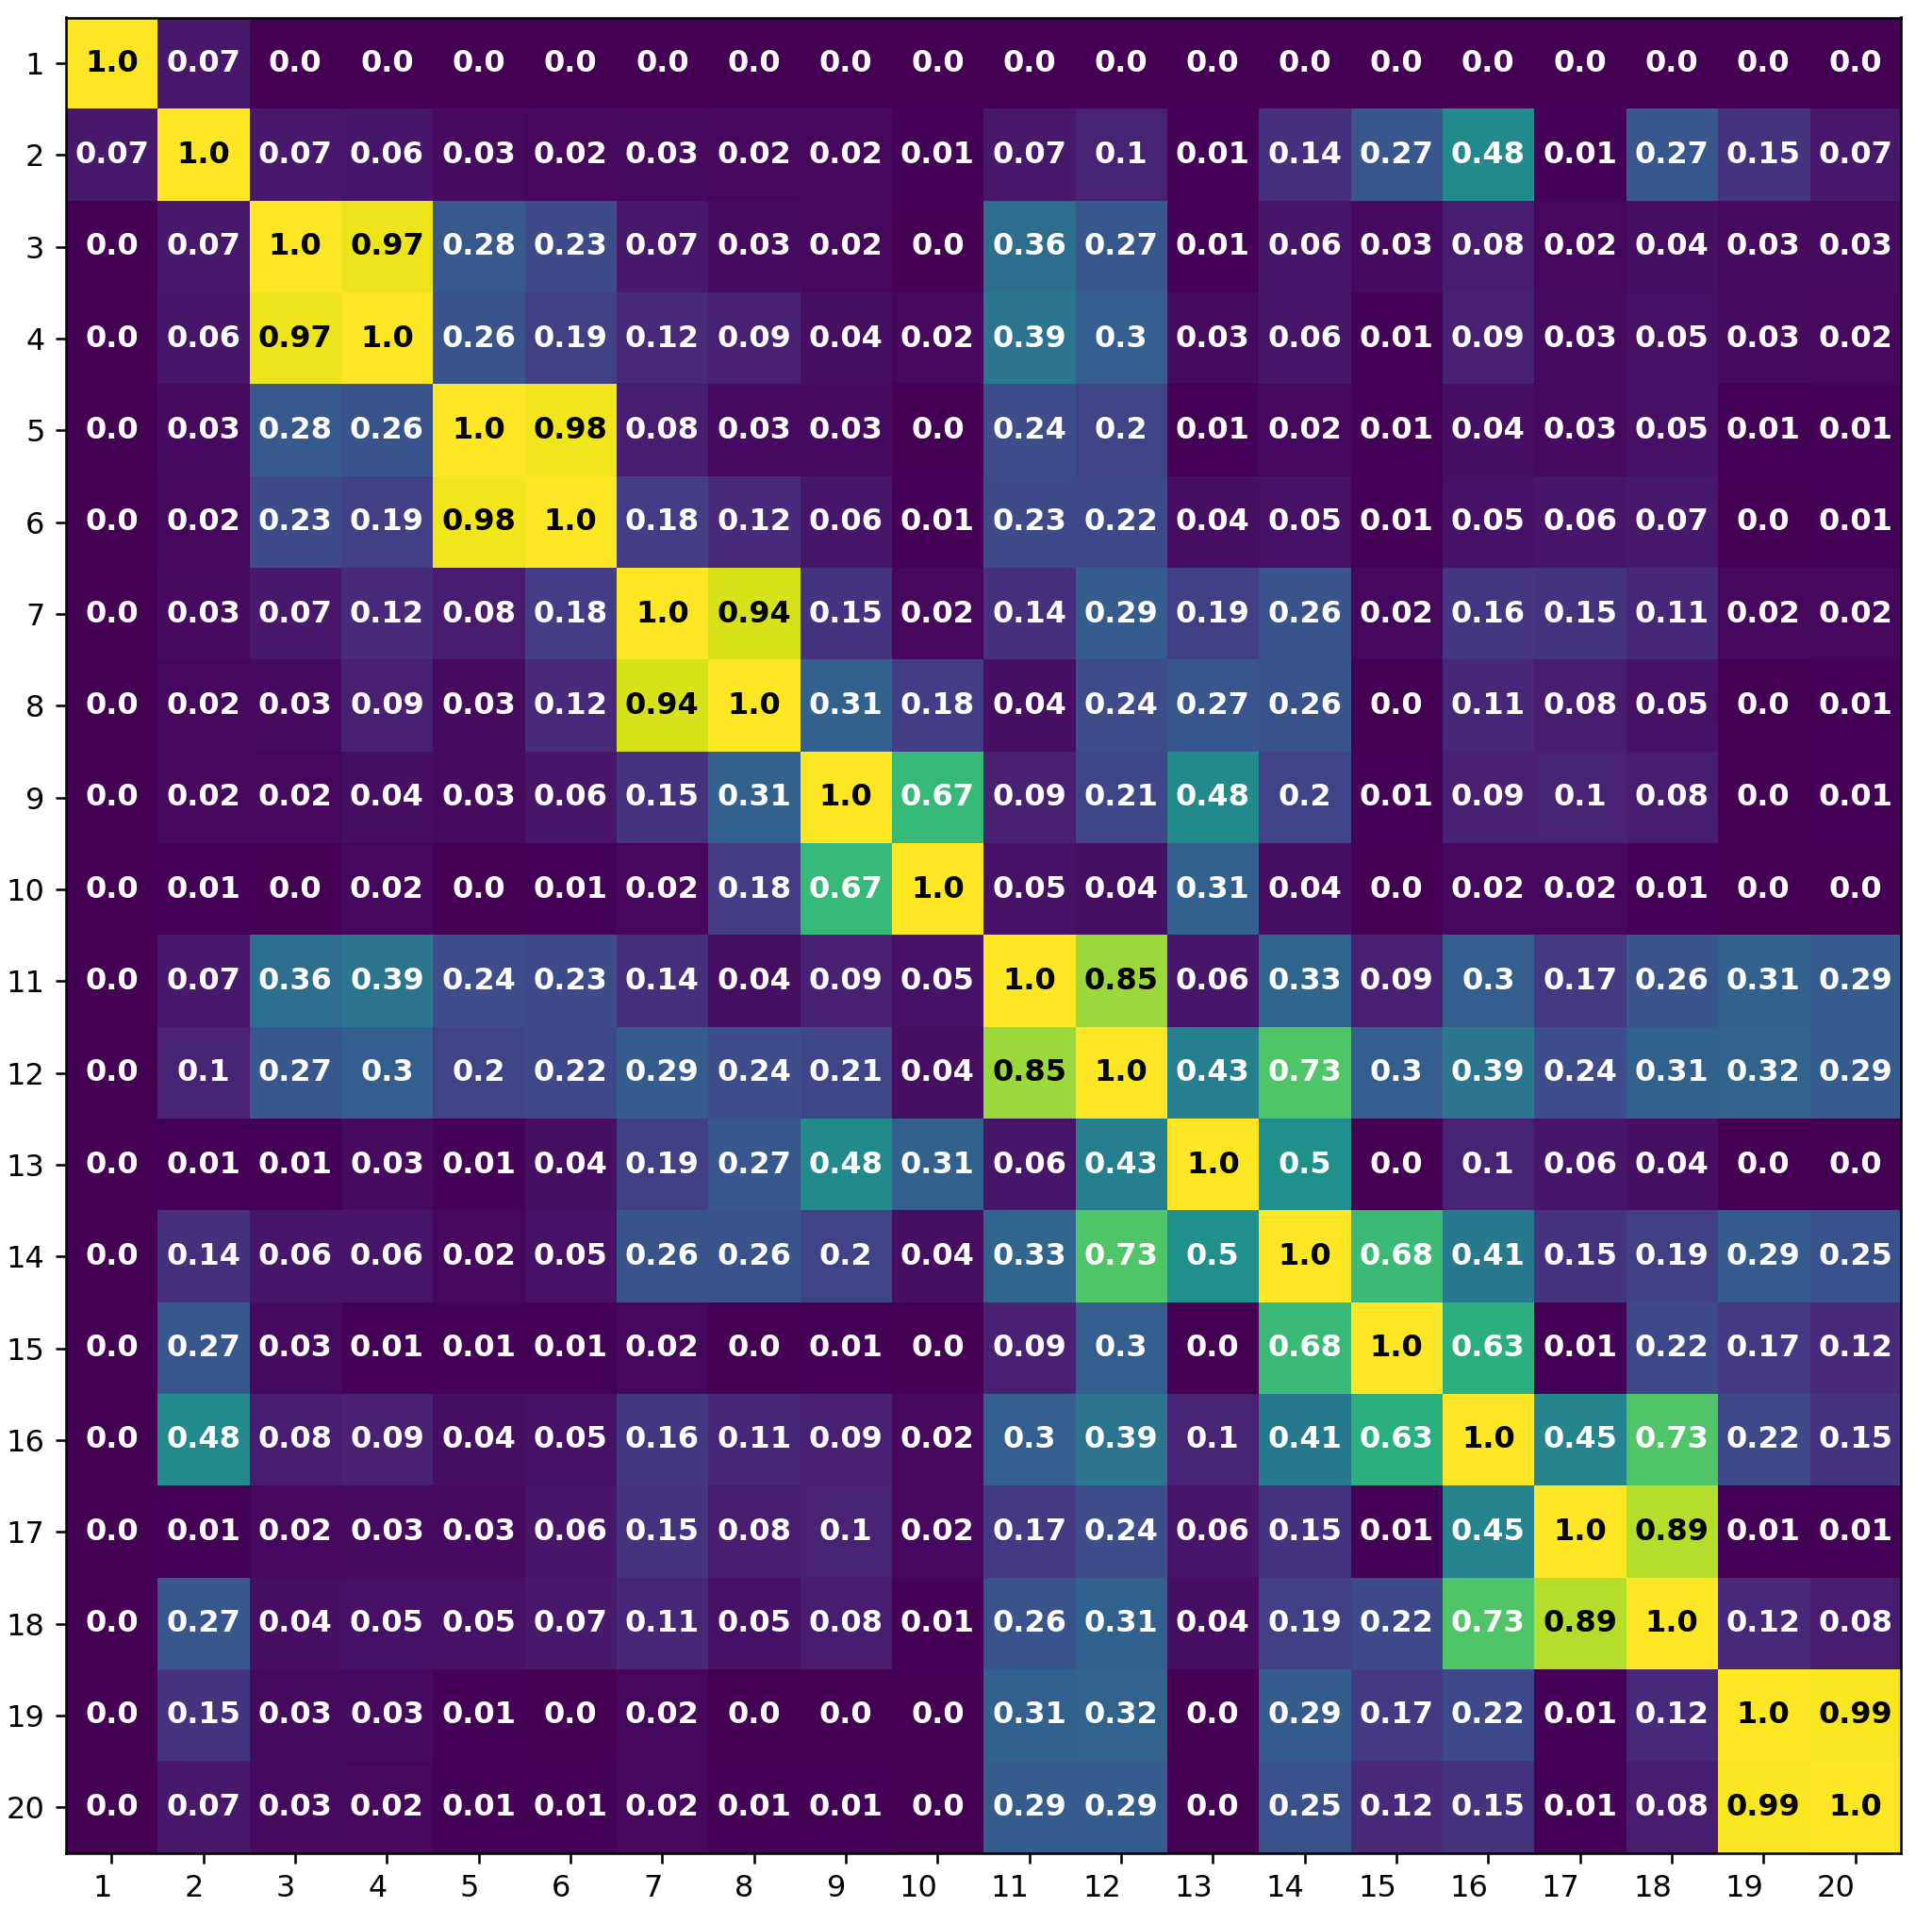
\includegraphics[width=16.5cm, height= 16.5cm]{ssa/W_corr.png}
	\caption{Корреляционная матрица компонент} \label{fig::W_corr_ssa}
\end{figure}

\noindent Финальным пунктом в примере классического SSA является демонстрация его предсказательных способностей.
\begin{figure}[H]
	\centering
	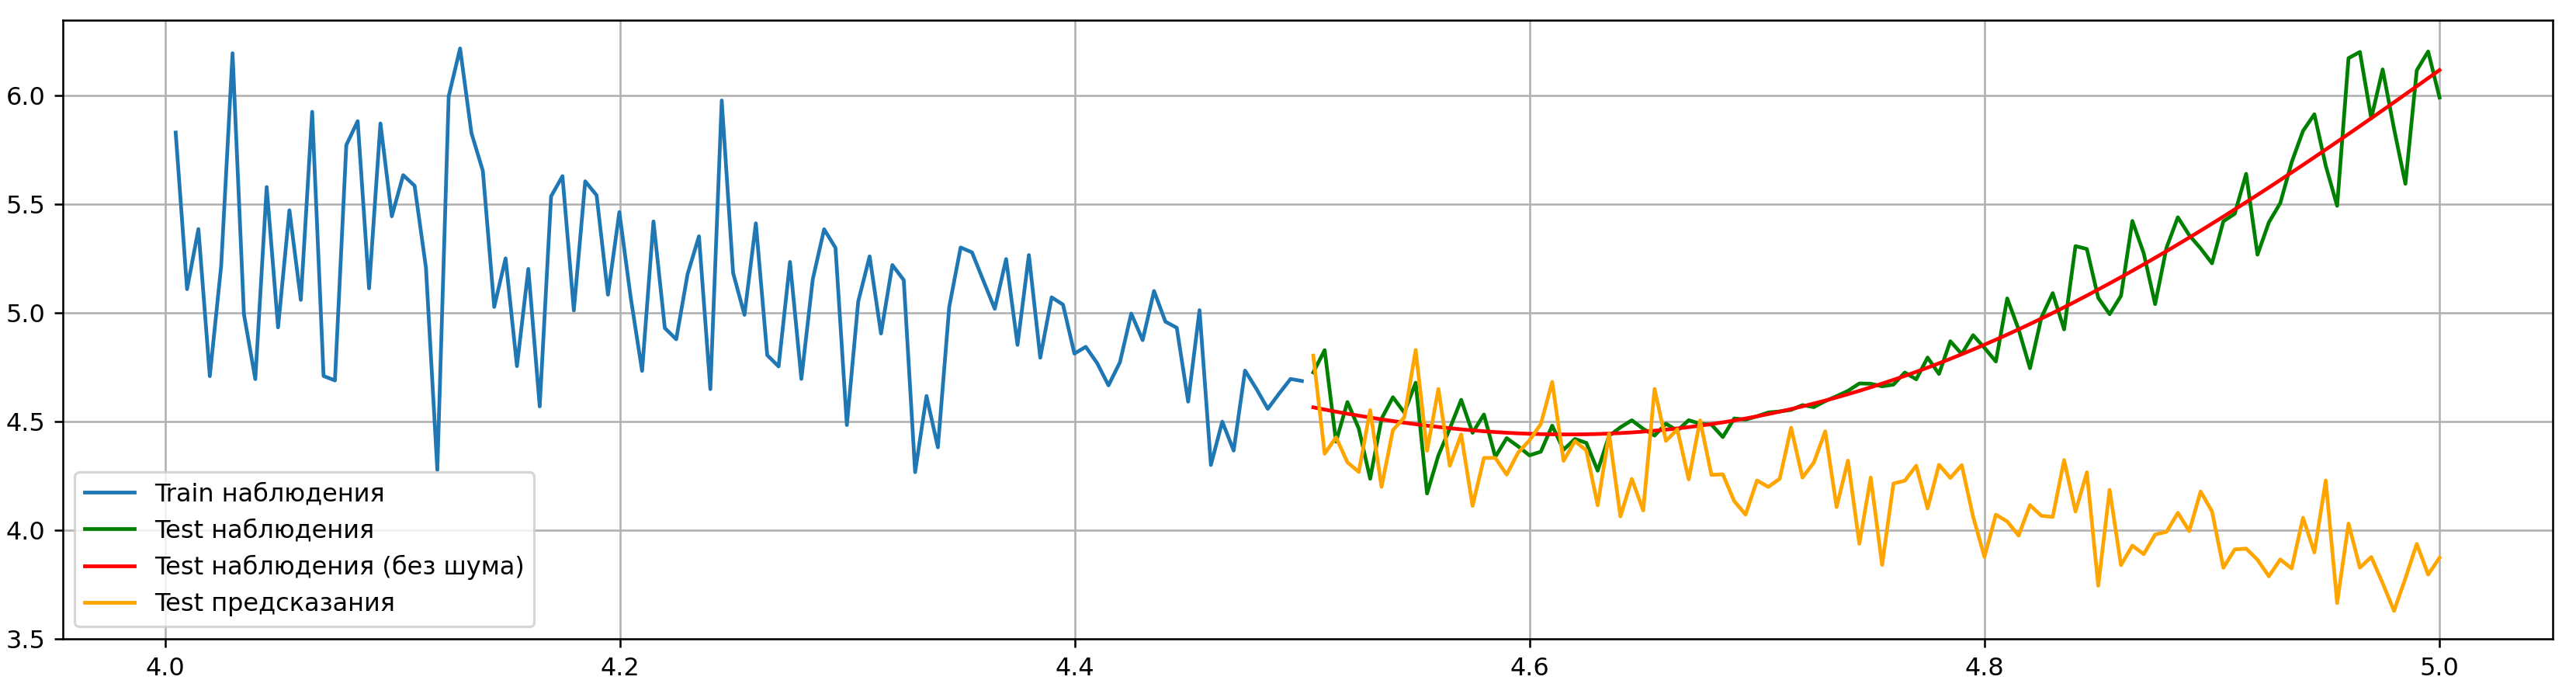
\includegraphics[width=16.5cm]{ssa/forecast_100.png}
	\caption{Прогнозирование значений $f(x)$ на ближайшие $100$ шагов}
\end{figure}
\noindent Анализируя полученные прогнозы, видим, что на начальных этапах они не очень плохи, однако дальше происходит расхождение самого тренда, что в случае с финансовыми рядами, влечет за собой большие риски (под риском понимается потеря денежного эквивалента из-за плохого расчета). Подобная ситуация случилась по 3-м причинам: 1) Малое количество компонент для деления 2) Отсутствие точного алгоритма группировки компонент 3) SSA не использует информацию о самом ряде, что анализирует, а опирается только на техническую составляющую. Однако 1) не говорит, что необходимо дробить ряд на как можно больше компонент, так как данный метод как и любой алгоритм требует как вычислительных мощностей, так и объемов оперативной памяти со стороны персонального компьютера. 2) не утверждает вообще ничего, а 3) упирается к гипотезу о рыночной эффективности и факт, что только техническим анализом невозможно точно предсказать поведение как цены, так и доходности актива соответственно \cite{fama_market_efficiency}. Конечно, 1-3 не утверждают, что SSA не применим вообще, иначе в чем смысл был смысл его создания. Решение - применять SSA конкретно для того, для чего он создавался: для анализа временных рядов - их декомпозиции и аппроксимации. то есть комбинировать его с другими алгоритмами, например, с NN или ARFIMA и так далее везде, где предсказывающая модель чувствительна к шуму в исходных данных. 